% Options for packages loaded elsewhere
\PassOptionsToPackage{unicode}{hyperref}
\PassOptionsToPackage{hyphens}{url}
%
\documentclass[
  letterpaper,
  DIV=11,
  numbers=noendperiod]{scrartcl}

\usepackage{amsmath,amssymb}
\usepackage{iftex}
\ifPDFTeX
  \usepackage[T1]{fontenc}
  \usepackage[utf8]{inputenc}
  \usepackage{textcomp} % provide euro and other symbols
\else % if luatex or xetex
  \usepackage{unicode-math}
  \defaultfontfeatures{Scale=MatchLowercase}
  \defaultfontfeatures[\rmfamily]{Ligatures=TeX,Scale=1}
\fi
\usepackage{lmodern}
\ifPDFTeX\else  
    % xetex/luatex font selection
\fi
% Use upquote if available, for straight quotes in verbatim environments
\IfFileExists{upquote.sty}{\usepackage{upquote}}{}
\IfFileExists{microtype.sty}{% use microtype if available
  \usepackage[]{microtype}
  \UseMicrotypeSet[protrusion]{basicmath} % disable protrusion for tt fonts
}{}
\makeatletter
\@ifundefined{KOMAClassName}{% if non-KOMA class
  \IfFileExists{parskip.sty}{%
    \usepackage{parskip}
  }{% else
    \setlength{\parindent}{0pt}
    \setlength{\parskip}{6pt plus 2pt minus 1pt}}
}{% if KOMA class
  \KOMAoptions{parskip=half}}
\makeatother
\usepackage{xcolor}
\setlength{\emergencystretch}{3em} % prevent overfull lines
\setcounter{secnumdepth}{-\maxdimen} % remove section numbering
% Make \paragraph and \subparagraph free-standing
\makeatletter
\ifx\paragraph\undefined\else
  \let\oldparagraph\paragraph
  \renewcommand{\paragraph}{
    \@ifstar
      \xxxParagraphStar
      \xxxParagraphNoStar
  }
  \newcommand{\xxxParagraphStar}[1]{\oldparagraph*{#1}\mbox{}}
  \newcommand{\xxxParagraphNoStar}[1]{\oldparagraph{#1}\mbox{}}
\fi
\ifx\subparagraph\undefined\else
  \let\oldsubparagraph\subparagraph
  \renewcommand{\subparagraph}{
    \@ifstar
      \xxxSubParagraphStar
      \xxxSubParagraphNoStar
  }
  \newcommand{\xxxSubParagraphStar}[1]{\oldsubparagraph*{#1}\mbox{}}
  \newcommand{\xxxSubParagraphNoStar}[1]{\oldsubparagraph{#1}\mbox{}}
\fi
\makeatother


\providecommand{\tightlist}{%
  \setlength{\itemsep}{0pt}\setlength{\parskip}{0pt}}\usepackage{longtable,booktabs,array}
\usepackage{calc} % for calculating minipage widths
% Correct order of tables after \paragraph or \subparagraph
\usepackage{etoolbox}
\makeatletter
\patchcmd\longtable{\par}{\if@noskipsec\mbox{}\fi\par}{}{}
\makeatother
% Allow footnotes in longtable head/foot
\IfFileExists{footnotehyper.sty}{\usepackage{footnotehyper}}{\usepackage{footnote}}
\makesavenoteenv{longtable}
\usepackage{graphicx}
\makeatletter
\def\maxwidth{\ifdim\Gin@nat@width>\linewidth\linewidth\else\Gin@nat@width\fi}
\def\maxheight{\ifdim\Gin@nat@height>\textheight\textheight\else\Gin@nat@height\fi}
\makeatother
% Scale images if necessary, so that they will not overflow the page
% margins by default, and it is still possible to overwrite the defaults
% using explicit options in \includegraphics[width, height, ...]{}
\setkeys{Gin}{width=\maxwidth,height=\maxheight,keepaspectratio}
% Set default figure placement to htbp
\makeatletter
\def\fps@figure{htbp}
\makeatother

\KOMAoption{captions}{tableheading}
\makeatletter
\@ifpackageloaded{caption}{}{\usepackage{caption}}
\AtBeginDocument{%
\ifdefined\contentsname
  \renewcommand*\contentsname{Table of contents}
\else
  \newcommand\contentsname{Table of contents}
\fi
\ifdefined\listfigurename
  \renewcommand*\listfigurename{List of Figures}
\else
  \newcommand\listfigurename{List of Figures}
\fi
\ifdefined\listtablename
  \renewcommand*\listtablename{List of Tables}
\else
  \newcommand\listtablename{List of Tables}
\fi
\ifdefined\figurename
  \renewcommand*\figurename{Figure}
\else
  \newcommand\figurename{Figure}
\fi
\ifdefined\tablename
  \renewcommand*\tablename{Table}
\else
  \newcommand\tablename{Table}
\fi
}
\@ifpackageloaded{float}{}{\usepackage{float}}
\floatstyle{ruled}
\@ifundefined{c@chapter}{\newfloat{codelisting}{h}{lop}}{\newfloat{codelisting}{h}{lop}[chapter]}
\floatname{codelisting}{Listing}
\newcommand*\listoflistings{\listof{codelisting}{List of Listings}}
\makeatother
\makeatletter
\makeatother
\makeatletter
\@ifpackageloaded{caption}{}{\usepackage{caption}}
\@ifpackageloaded{subcaption}{}{\usepackage{subcaption}}
\makeatother

\ifLuaTeX
  \usepackage{selnolig}  % disable illegal ligatures
\fi
\usepackage{bookmark}

\IfFileExists{xurl.sty}{\usepackage{xurl}}{} % add URL line breaks if available
\urlstyle{same} % disable monospaced font for URLs
\hypersetup{
  pdftitle={30538 Final Project: Reproducible Research - Volunteerism, Engagement, and Polarization in the U.S.},
  pdfauthor={Andrew White, Charles Huang, Justine Silverstein},
  hidelinks,
  pdfcreator={LaTeX via pandoc}}


\title{30538 Final Project: Reproducible Research - Volunteerism,
Engagement, and Polarization in the U.S.}
\author{Andrew White, Charles Huang, Justine Silverstein}
\date{2024-12-07}

\begin{document}
\maketitle


\section{1. Background}\label{background}

This project began as a shared interest in trends behind volunteering
rates in America, as two of our members (Justine and Charles) are
AmeriCorps alumni.

For the past few years, concerns about the American public's increasing
rates of isolation, decreasing lack of civic engagement and faith in
institutions, and greater rates of political polarization have been
prominent in the news and media. Our personal experiences with
AmeriCorps and volunteering have taught us that volunteering can be
effective at reducing isolation, increasing civic engagement/community
awareness, and decreasing negative polarization towards ``the other
side''. However, is volunteering a legitimate part of a public policy
solution to these issues, or is it just a red herring?

Our research questions were: 1. What is the current state of
volunteerism, political engagement and polarization in America? 2. What
factors make people more likely to volunteer or be civically engaged?

\section{2. Data Importing/Cleaning}\label{data-importingcleaning}

Our datasets for this project were:

\begin{enumerate}
\def\labelenumi{\arabic{enumi}.}
\tightlist
\item
  AmeriCorps CEV (Civic Engagement and Volunteering Supplement) for 2021
\item
  U.S. Census Bureau Volunteering and Civic Life (VCL) Supplement -
  September 2021
\item
  ANES (American National Election Studies) Time Series Data, 2020
\end{enumerate}

\#1 and \#2 primarily contain respondent information about volunteering
and measures of civic engagement, while \#3 contains information on
political affiliation and polarization.

We are importing the data from the AmeriCorps and ANES websites. Because
the datasets are over 100 MB, we include a Google Drive link here:

https://drive.google.com/drive/folders/1PUTN2pyh78MLoK0RVtGnf1ZwiM1BAAuV?usp=sharing

As there are over 400 variables in the CEV and VCL data, we focused on
the 20 most relevant variables in the following categories:

\begin{enumerate}
\def\labelenumi{\arabic{enumi}.}
\tightlist
\item
  Frequency and Type of Volunteering
\item
  Political Engagement (did respondents discuss politics, did they write
  to elected officials, boycott products, etc.)
\item
  Civic/Community Participation (did respondents belong to
  groups/associations, interact with neighbors, etc.)
\item
  Basic demographics (age, gender, race, income, education, etc.)
\end{enumerate}

Because the CEV and VCL data use similar variable names (by design), we
were able to merge the two datasets together after cleaning the column
names. Since the data values in the CEV/VCL data are entered in numeric
codes (-1, 1, 2, etc.), we also created mapping functions with
dictionaries to convert the data as needed.

(One notable issue we encountered with cleaning the CEV/VCL data was a
hetereogeneous mix of numeric code and qualitative input. We made an
additional helper function that identifies all the values in the data
that aren't picked up by our data dictionaries- this function is located
in our config.py file.)

\section{2b. Data cleaning - ANES
data}\label{b.-data-cleaning---anes-data}

As with the CEV/VCL data, our goal was to subset the data so that it
only contains relevant variables. We accomplished this by making two
lists- one designed to capture variables covering geographic information
(V201011, V201013a, V201013b, V201014a, V201014b), and one designed to
capture variables covering information about assessments of political
positioning (i.e.~left, right, center)

Similarly, we also used a mapping function to change numerical codes to
qualitative data in two relevant questions:

V201200 - ``Where would you place yourself on this {[}extremely liberal
to extremely conservative{]} scale, or haven't you thought much about
this?''

V201228 - ``Generally speaking, do you usually think of yourself as {[}a
Democrat, a Republican / a Republican, a Democrat{]}, an independent, or
something else?''

\section{3. Custom Variables}\label{custom-variables}

We devised two custom measures of political engagement and polarization
derived from the survey results:

I. Political Engagement Score

We chose five of the most relevant questions from the CEV/VCL data and
weighted each based on their level of effort:

\begin{enumerate}
\def\labelenumi{\arabic{enumi}.}
\tightlist
\item
  ``How frequently do you talk to a family member/neighbor about
  politics?'' (15\%)
\item
  ``How frequently do you post political views on social media?'' (15\%)
\item
  ``How frequently do you consume political news/media?'' (10\%)
\item
  ``Did you contact an elected official to express your opinion in the
  last 12 months?'' (30\%)
\item
  ``Did you boycott a company based on their values in the last 12
  months?'' (30\%)
\end{enumerate}

This generated a score from 0 - 100 that we could use as a (imperfect)
proxy for political engagement. We mutated a new variable to measure
this and added it to our dataset.

\begin{enumerate}
\def\labelenumi{\Roman{enumi}.}
\setcounter{enumi}{1}
\tightlist
\item
  Polarization Score
\end{enumerate}

In a paper on quantifying polarization written by Aaron Bramson et al
(https://inferenceproject.yale.edu/sites/default/files/688938.pdf), the
authors examine a range of polarization indicators. A relatively simple
(and in some ways problematic) measurement is called spread, or
dispersion. Bramson et al.~explain: ``Polarization\ldots can be measured
as the value of the agent with the highest belief value minus the value
of the agent with the lowest belief value.''

We (imperfectly) approximate this using two more variables: V201206 and
V201207. These ask respondents to position political parties on the
political spectrum. We selected the most ideologically distant nodes on
the personal ideology scale (extremely liberal and extremely
conservative) and capture how far apart their conceptions of each party
are, on average.

We created a scale to assign the different ideological positions on a
spectrum, namely: -3, -2, and -1 are ``Extremely Liberal'', ``Liberal'',
and ``Slightly Liberal''; 0 is ``Moderate; middle of the road''; 1, 2,
and 3 are ``Slightly conservative'', ``Conservative'', and ``Extremely
conservative.''

For example, if the average extremely liberal respondent in Texas places
Democrats at -1 (slightly liberal) and the average for the extremely
conservative respondents is 3 (extremely conservative), then the
distance between the two is 4, meaning Texas would have a spread of 4
for this question.

\section{4. Static Plots and Outcomes}\label{static-plots-and-outcomes}

\section{Caveats}\label{caveats}

Before discussing the data, we acknowledge we cannot discuss patterns
over time as we only have data from 2021 in the case of the AmeriCorps
and U.S. Census data, and 2020 in the case of the ANES data. However,
the data is still useful as we can garner a lot from even a snapshot in
time, especially as this was right after the height of the COVID
pandemic and a highly contentious election. Furthermore (as noted in the
shiny app), many entries were missing from the datasets due to
nonresponse. As an example, over 80\% respondents did not answer a
majority of our political engagement questions, forcing us to exclude
them from the analysis. While we believe our analyses still provide
useful information, this potential selection bias should be taken into
account.

\section{4a. Exploratory Analysis -
Volunteering}\label{a.-exploratory-analysis---volunteering}

When initially working with the data, we generated multiple plots with
different variables to see if we could notice any noteworthy trends
between volunteering frequency and civic indicators such as public
officials, boycotts, etc. (These charts are not shown here for space,
but the output is included in our code.)

As part of our exploratory analysis, we also ran a groupby on
state-level data to see if there was any correlation between the number
of volunteers per state and the average hours volunteered; however,
there did not seem to be any correlation between the two.

We want to highlight two charts out of the ones we produced. The first
chart depicts the top and bottom five states by average hours spent
volunteering:

\begin{figure}[H]

{\centering 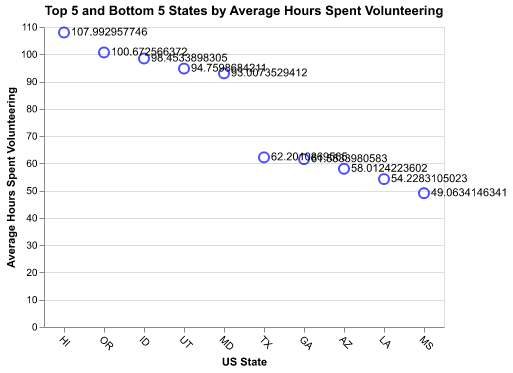
\includegraphics{top_bottom_5_states_avg_volunteering.png}

}

\caption{Top 5 and Bottom 5 US States by average hours spent
volunteering}

\end{figure}%

The second chart depicts volunteering frequency when measured against
voters and nonvoters:

\begin{figure}[H]

{\centering 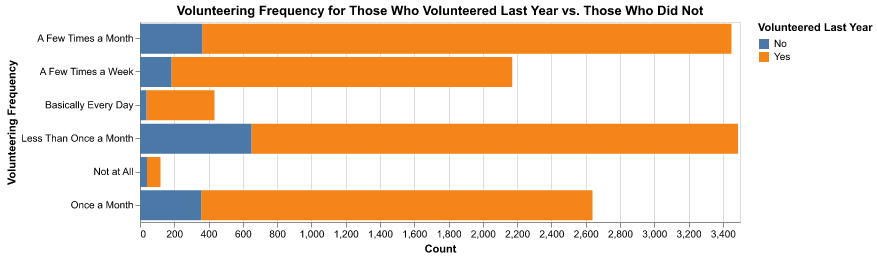
\includegraphics{if_volunteered_last_year.png}

}

\caption{Volunteering Frequency for Voters and Non-Voters}

\end{figure}%

An interesting point from our exploratory analysis is that in each
volunteering category, the majority of people did vote in their local
election. However, it is unclear if this is simply correlation, as
AmeriCorps may disproportionately attract the kind of person already
primed to vote in their local election and be politically engaged. We
will engage this question of correlation further with our Shiny app
results.

\section{4b. Polarization Analysis}\label{b.-polarization-analysis}

With the ANES data, we focused more specifically on measuring political
polarization, to try to examine our hypothesis that volunteering would
correlate negatively with polarization.

As mentioned above, we devised a simple ``spread'' variable from Bramson
et al.~to measure polarization. We then graphed each state's spread
alongside average political engagement score and average volunteer
hours. As an example, here is a graph of spread of views on Democrat
Party ideological position, including volunteering hours:

\begin{figure}[H]

{\centering 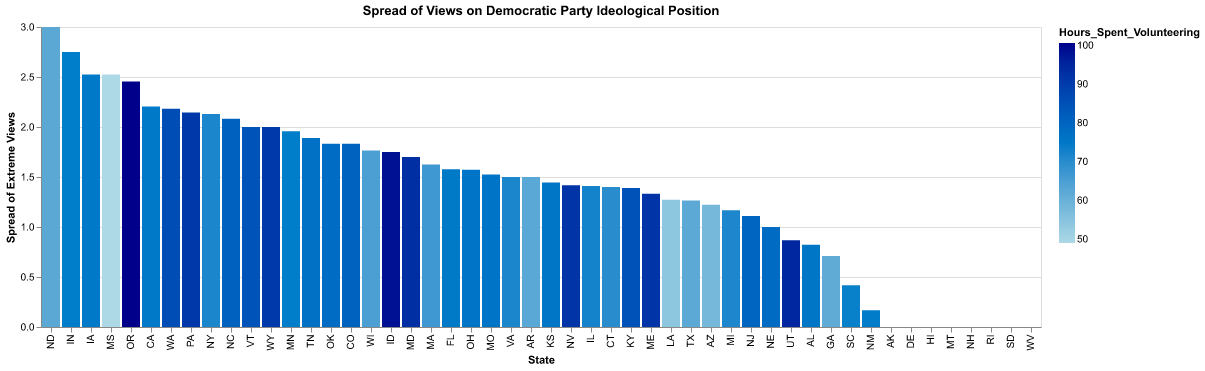
\includegraphics{dem_graph_spread_2.png}

}

\caption{Spread of views on Democrat Party}

\end{figure}%

We found that these graphs do not appear to show a significant
meaningful correlation between extreme views and volunteering in either
Democrat or Republican analyses; we may have chosen some of the states
with very high or very low spread, and it is clear that there is not
much of a relationship, with high spread being found in some
higher-volunteer states and some lower-volunteer states.

In the future, causal techniques such as regression analysis with
controls for potential bias coming from variables such as income and
education, or a difference-in-differences approach examining specific
states over time, could better help to precisely measure polarization
alongside political engagement.

\section{5. Dynamic Plots in Shiny - Demographics vs.~Volunteering
Rate/Political
Engagement}\label{dynamic-plots-in-shiny---demographics-vs.-volunteering-ratepolitical-engagement}

Building off of our exploratory analysis, we wanted to more easily see
the correlations between volunteerism, political engagement, and
potential confounders like income and education. We made a Shiny
dashboard app using the CEV/VCL data that lets us see demographics (age,
education level, income, US state, etc.) on the X-axis and the user's
choice of volunteer rates or political engagement on the Y-axis.

A screenshot of the app is here: 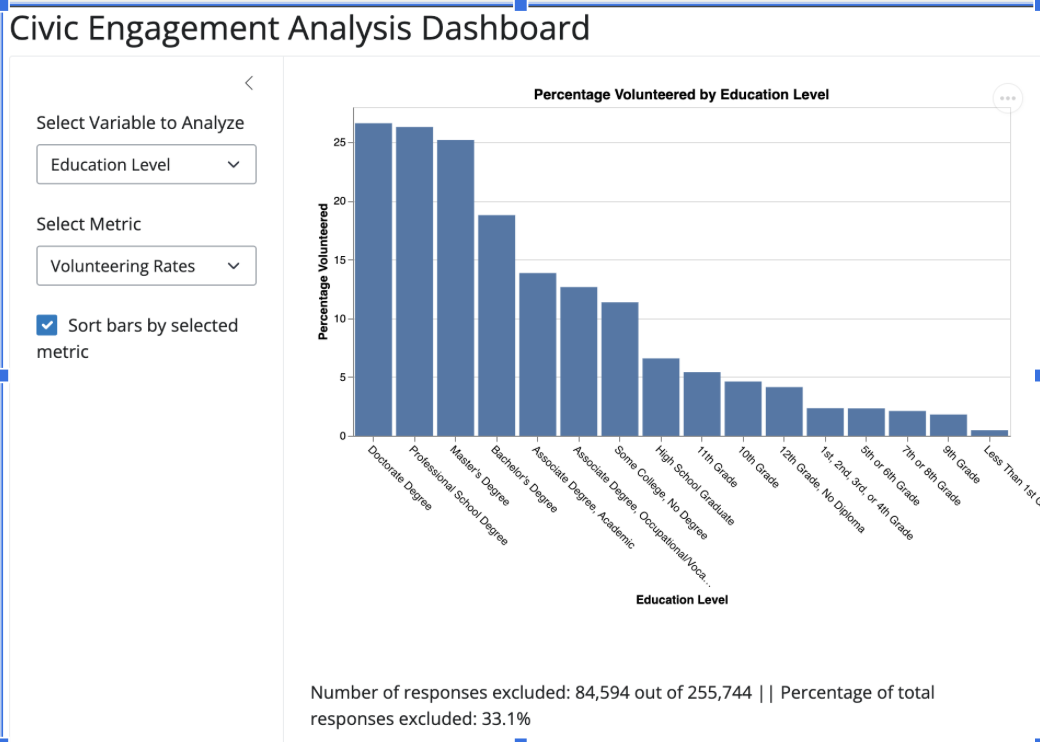
\includegraphics{shiny_screenshot.png}

As an example, we can see here that volunteering is positively
correlated with educational attainment, with over 25\% of
PhD/professional/master's degree holders having volunteered in 2021.

Using this app, we were able to find the most common traits associated
with volunteering and civic engagement for 2021: family income and
education, marital status, age, and being of White or Native
American/Alaskan Indian heritage.

We also found that women and rural inhabitants were slightly more likely
to volunteer than men/urban inhabitants, but civic engagement remained
the same. Additionally (but not surprisingly) social media was a
negative predictor of volunteering, but not civic engagement.

This analysis reveals something critical about our hypothesis- while
volunteering can still be a solution to low civic engagement, we can't
dismiss that both are simply correlated with other overarching
demographic factors like income, education, and race, which makes sense
as those factors can indicate well-off people having more resources and
time to volunteer than others.

\section{6. Conclusion/Takeaways}\label{conclusiontakeaways}

As mentioned before, our data and analysis has several disclaimers and
caveats that we cannot fully account for. Nevertheless, our takeaways
are here in order:

\begin{enumerate}
\def\labelenumi{\arabic{enumi}.}
\tightlist
\item
  Volunteers are more likely to vote than non-volunteers, but this is
  less likely to be a causation and more a correlation of demographic
  factors
\item
  We did not find a meaningful correlation between volunteering and
  polarized attitudes; the evidence that volunteering in particular has
  a positive effect on polarization and engagement seems weak.
\item
  We found that predictors of volunteering and civic engagement are
  concentrated in disproportionately well-off, privileged populations.
\end{enumerate}

For organizations like AmeriCorps that want to attract younger or more
diverse volunteers, as well as improving civic participation/engagement
in general, this has important implications- organizations like those
should consider that simple appeals to volunteer more, or attempts to
diversify volunteer populations, may not mean much without additional
incentives that can address the structural barriers of volunteering.

While volunteering can still be a solution to low civic engagement, and
we can speak personally to its interpersonal benefits, we can't dismiss
that both are simply correlated with other overarching demographic
factors like income, education, and race. This should give us pause to
the theory that volunteering is a neat solution to reducing polarization
and improving civic engagement in and of itself, but future studies can
examine specific populations of low-income or other ``non-typical''
volunteers that reported positive outcomes- perhaps volunteering itself
has certain aspects (like community, sense of purpose, etc.) that can
still be valuable regardless of socioeconomic status.

\section{7. Coding Analysis (Not Shown in
Writeup)}\label{coding-analysis-not-shown-in-writeup}

We will use two measures of polarization from the ANES data; each
provides some amount of information that can be interpreted to indicate
polarization to a certain extent, though both have their drawbacks.

\begin{enumerate}
\def\labelenumi{\arabic{enumi}.}
\tightlist
\item
  Share of Outliers - we create a series of functions that group
  respondents by party Democrats with conservative-leaning ideologies,
  and Republicans with liberal-leaning ones.
\end{enumerate}

\section{the following chart is total number of volunteers per state and
stacked by volunteer
frequency}\label{the-following-chart-is-total-number-of-volunteers-per-state-and-stacked-by-volunteer-frequency}

\section{same as above except now if person contacted public
official}\label{same-as-above-except-now-if-person-contacted-public-official}




\end{document}
